\chapter{\IfLanguageName{dutch}{Stand van zaken}{State of the art}}%
\label{ch:stand-van-zaken}
% Tip: Begin elk hoofdstuk met een paragraaf inleiding die beschrijft hoe
% dit hoofdstuk past binnen het geheel van de bachelorproef. Geef in het
% bijzonder aan wat de link is met het vorige en volgende hoofdstuk.

% Pas na deze inleidende paragraaf komt de eerste sectiehoofding.

\section{Inleiding tot CI/CD en DevOps}

De concepten Continuous Integration (CI) en Continuous Deployment (CD) zijn fundamenteel geworden in moderne softwareontwikkelingspraktijken. Deze methodologieën bieden organisaties de mogelijkheid om software op een snellere, meer betrouwbare en schaalbare manier te ontwikkelen en uit te rollen. CI/CD vormt een kerncomponent van DevOps, een filosofie en praktijk die gericht is op nauwe samenwerking tussen ontwikkelings- en operationele teams om de levering van software te versnellen en de kwaliteit te verbeteren.

\subsection{Wat is Continuous Integration (CI)?}
Continuous Integration is een softwareontwikkelingspraktijk waarbij ontwikkelaars regelmatig wijzigingen integreren in een gedeelde repository. Dit proces wordt ondersteund door geautomatiseerde builds en tests die ervoor zorgen dat nieuwe wijzigingen consistent blijven met de bestaande code. Volgens Marques en Correia \autocite{marques2023} minimaliseert CI de risico's op integratieproblemen door foutdetectie vroeg in de ontwikkelingscyclus mogelijk te maken. Voordelen van CI zijn:
\begin{itemize}
    \item Snelle feedback loops: Problemen worden vroegtijdig opgespoord en opgelost.
    \item Efficiënt samenwerken: Ontwikkelaars werken op een uniforme codebase.
    \item Stabiele builds: Automatische tests garanderen dat code stabiel blijft .
\end{itemize}

\subsection{Wat is Continuous Deployment (CD)?}
Continuous Deployment bouwt voort op Continuous Integration (CI) door geautomatiseerde uitrol naar productie mogelijk te maken. Wanneer codewijzigingen alle tests succesvol doorlopen, worden ze automatisch geïmplementeerd in de productieomgeving. Dit versnelt de time-to-market en elimineert menselijke fouten in het uitrolproces. \autocite{Learn2024}

Belangrijke voordelen van CD zijn:

\begin{itemize}
    \item Consistentie in uitrol: Door automatisering zijn uitrolprocessen reproduceerbaar en minder foutgevoelig.
    \item Hogere snelheid: Functionaliteiten en bugfixes zijn sneller beschikbaar voor eindgebruikers.
    \item Kostenbesparing: Minder menselijke tussenkomst leidt tot lagere kosten en een efficiënter proces.
\end{itemize}

\subsection{De rol van CI/CD in DevOps}
CI/CD is een integraal onderdeel van de bredere DevOps-filosofie, die gericht is op het elimineren van silo's tussen ontwikkeling (Dev) en operations (Ops). DevOps streeft naar snellere en betrouwbaardere leveringen van software door middel van samenwerking en automatisering. Zoals Marques en Correia \autocite{marques2023} aangeven, ondersteunen CI/CD-processen dit doel door continue iteraties, geautomatiseerde kwaliteitscontroles en snellere terugkoppeling.

Enkele belangrijke voordelen in deze context zijn:
\begin{itemize}
    \item Automatisering: Bouw-, test- en implementatieprocessen worden gestroomlijnd, wat de ontwikkelingssnelheid verhoogt.
    \item Iteratieve verbeteringen: Kleine, frequente wijzigingen verminderen de kans op grootschalige fouten.
    \item Hogere betrouwbaarheid: Geautomatiseerde pipelines minimaliseren de kans op menselijke fouten en vergroten de stabiliteit van de applicatie.
\end{itemize}


\subsection{uitdagingen in CI/CD}
Hoewel CI/CD aanzienlijke voordelen biedt, brengt de implementatie ervan ook uitdagingen met zich mee:
\begin{itemize}
    \item Complexiteit: Het opzetten van geautomatiseerde pipelines vereist technische expertise en een zorgvuldige architectuur. \autocite{Learn2024}
    \item Beveiliging: Het veilig beheren van secrets, zoals API-sleutels en wachtwoorden, blijft een belangrijke uitdaging. Moderne CI/CD-tools bieden functionaliteiten zoals secret management, maar verkeerde configuraties kunnen risico's introduceren. \autocite{atlassian2024}
    \item Toolselectie: Er is een breed scala aan CI/CD-tools beschikbaar, elk met unieke kenmerken. Het kiezen van een oplossing die past bij de specifieke eisen van een organisatie vereist grondig onderzoek. \autocite{true_cicd2024}
\end{itemize}


\subsection{De toekomst van CI/CD in DevOps}
De toekomst van CI/CD richt zich op integratie met beveiligingspraktijken (DevSecOps) en de toepassing van machine learning in geautomatiseerde pipelines. DevSecOps stelt organisaties in staat om beveiligingstests en compliancechecks vroeg en vaak in de ontwikkelingscyclus uit te voeren. Daarnaast zal machine learning naar verwachting processen zoals foutdetectie en resource-optimalisatie verder verbeteren. \autocite{marques2023}

\subsection{Overzicht van de CI/CD pijplijn}

\begin{figure}[h!]
    \centering
    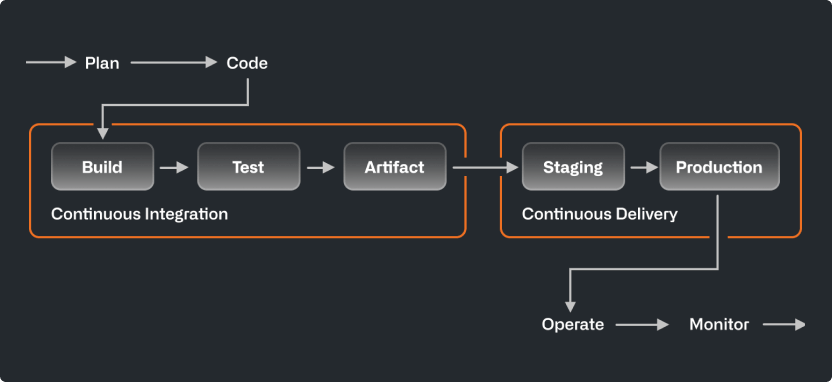
\includegraphics[width=\linewidth]{"C:/Users/laure/Documents/bachelorproef-2024-2025-laurensDeVos/graphics/cicd-pipeline.png"}
    \caption{Overzicht van een typische CI/CD-pijplijn}
    \label{fig:cicd-pipeline}
    \autocite{GitHub2022}
\end{figure}


\section{Evaluatiecriteria}

Het selecteren van een CI/CD-tool vereist een gestructureerde evaluatie van kritieke criteria die aansluiten bij de operationele en strategische behoeften van een organisatie. In deze sectie worden vijf kerncriteria besproken die organisaties kunnen helpen bij het kiezen van de juiste CI/CD-oplossing. De besproken criteria zijn gebaseerd op een combinatie van academisch onderzoek en industriële inzichten.

\subsection{Prestaties}
De prestaties van een CI/CD-tool bepalen hoe efficiënt en betrouwbaar build- en deploymentprocessen worden uitgevoerd. Shahin et al. \autocite{shahin2017} benadrukken dat snellere buildtijden en verbeterde schaalbaarheid cruciaal zijn voor moderne softwareontwikkeling.
Belangrijke factoren die bijdragen aan de prestaties zijn: \begin{itemize} \item Build- en testtijden: Kortere cyclustijden verbeteren de feedbackloop voor ontwikkelaars en verhogen de productiviteit. \item Schaalbaarheid: Tools moeten effectief omgaan met groeiende workloads, zoals meerdere parallelle builds of grotere codebases. Dit is vooral belangrijk voor organisaties met een hoge releasefrequentie. \autocite{springer2023ci} \item Betrouwbaarheid: Een tool met een hoge uptime en fouttolerantie minimaliseert onderbrekingen in de workflow. \autocite{ieee2021cicd} \end{itemize}

\subsection{Beveiliging}
Beveiliging is een kernoverweging bij het implementeren van CI/CD-tools. Een goed beveiligde tool vermindert risico's zoals gegevenslekken en biedt ondersteuning voor compliance met regelgeving zoals GDPR en ISO 27001. Volgens J. Smith en collega's \autocite{smith2023securityci} moeten organisaties letten op:
\begin{itemize} 
    \item Secrets management: Veilige opslag en beheer van gevoelige gegevens, zoals API-sleutels, is essentieel. Jenkins en GitHub Actions bieden geïntegreerde oplossingen zoals Credentials Plugin en GitHub Secrets voor versleutelde opslag van gegevens \autocite{githubdocs2023secrets}.
    \item Beveiligingsintegratie: Tools moeten beveiligingscontroles zoals vulnerability scanning en dependency-checks ondersteunen. Integratie met tools zoals SonarQube en OWASP ZAP helpt bij het vroegtijdig identificeren van kwetsbaarheden \autocite{owasp2023}.
    \item Audit logs: Logging van acties binnen de pipeline stelt organisaties in staat om verdachte activiteiten te detecteren en te rapporteren. Moderne CI/CD-tools ondersteunen uitgebreide loggingfuncties om compliance te vergemakkelijken \autocite{forsgren2018}.
\end{itemize}

\subsection{Automatiseringsefficiëntie}

Volgens recente studies \autocite{forsgren2018, githubdocs2023actions} is automatiseringsefficiëntie een sleutelcriterium bij het selecteren van CI/CD-tools. Belangrijke aspecten zijn:
\begin{itemize}
    \item \textbf{Configuratiegemak}: Tools met intuïtieve interfaces en duidelijke documentatie verminderen de leercurve en vergemakkelijken implementatie. Jenkins biedt flexibiliteit via declaratieve pijplijnen, terwijl GitHub Actions YAML-gebaseerde configuratie aantrekkelijk maakt voor minder ervaren gebruikers \autocite{forsgren2018}.
    \item \textbf{Herbruikbare componenten}:De mogelijkheid om gedeelde configuraties en sjablonen te gebruiken verhoogt de efficiëntie. Jenkins ondersteunt grootschalige herbruikbare configuraties via shared libraries, terwijl GitHub Actions een uitgebreide Marketplace biedt met herbruikbare workflows \autocite{githubdocs2023marketplace}.
    \item \textbf{Integratie met testtools}: Naadloze integratie met frameworks zoals Selenium, JUnit en Pytest stelt ontwikkelaars in staat om tests volledig te automatiseren en snel feedback te ontvangen \autocite{smith2023automation}.
\end{itemize}


\subsection{Integratie met bestaande systemen}
Een CI/CD-tool moet naadloos integreren met de bestaande infrastructuur en tooling van een organisatie. Shahin et al. \autocite{shahin2017} benadrukken dat compatibiliteit met tools zoals versiebeheer, containerplatforms en cloudservices van cruciaal belang is voor een soepele workflow.
Belangrijke integratiecriteria zijn: \begin{itemize} \item Versiebeheersystemen: Ondersteuning voor Git en andere versiebeheertools is essentieel. \autocite{springer2023ci} \item Container- en cloudondersteuning: Integratie met Docker, Kubernetes, en cloudproviders zoals AWS en Azure maakt flexibele implementaties mogelijk. \autocite{ieee2021cicd} \item Third-party tools: Compatibiliteit met projectmanagementtools zoals JIRA of monitoringtools zoals Prometheus verhoogt de productiviteit. \end{itemize}

\subsection{Kosten}
De totale kosten van een CI/CD-tool omvatten niet alleen licenties, maar ook infrastructuur, onderhoud en training. Volgens een studie in IEEE Xplore \autocite{ieee2023costbenefit} moeten organisaties rekening houden met: \begin{itemize} \item Licentiekosten: Sommige tools zijn open-source en gratis, terwijl andere abonnementen of op gebruik gebaseerde kosten vereisen. \item Onderhoud en infrastructuur: Self-hosted oplossingen brengen extra server- en onderhoudskosten met zich mee. \item Return on Investment (ROI): De efficiëntie en tijdsbesparing die een tool biedt, moeten opwegen tegen de initiële en doorlopende kosten. \end{itemize}
 
\section{Beschrijving van Jenkins}

Jenkins is een open-source automatiseringsserver die zich heeft gevestigd als een hoeksteen in de wereld van Continuous Integration (CI) en Continuous Deployment (CD). Sinds de lancering in 2011 heeft het een sterke positie verworven dankzij zijn uitgebreide functionaliteit en flexibiliteit. Jenkins biedt ontwikkelaars de mogelijkheid om wijzigingen in code continu te integreren, geautomatiseerde tests uit te voeren en betrouwbare softwarelevering te waarborgen \autocite{shahin2017}.

\subsection{Architectuur van Jenkins}

De architectuur van Jenkins is ontworpen met schaalbaarheid en flexibiliteit in gedachten. Het volgt een \textit{master-agent} model:
\begin{itemize}
    \item \textbf{Master}: De Jenkins-master beheert CI/CD-pijplijnen, coördineert taken en fungeert als controlepunt voor de gebruikersinterface. De master verwerkt ook configuraties, zoals Jenkinsfiles, waarin pijplijnstappen declaratief worden beschreven.
    \item \textbf{Agents}: Deze zijn verantwoordelijk voor het uitvoeren van taken zoals builds, tests en implementaties. Jenkins ondersteunt zowel statische agents (toegewijd aan specifieke taken) als dynamische agents die worden opgeroepen op basis van behoeften. Deze flexibiliteit maakt Jenkins geschikt voor kleine projecten en grote, complexe workflows \autocite{springer2023ci}.
\end{itemize}

De architectuur ondersteunt ook integratie met containertechnologieën zoals Docker en orchestrators zoals Kubernetes, wat het geschikt maakt voor cloud-native applicaties \autocite{amaral2021}.

\subsection{Functionaliteiten en Sterke Punten}

Jenkins biedt een breed scala aan functionaliteiten die het tot een van de meest gebruikte CI/CD-tools maken:
\begin{itemize}
    \item \textbf{Plugin-ecosysteem}: Met meer dan 1.800 plugins biedt Jenkins integraties met tools zoals Git, Docker, Maven en Slack. Dit maakt het mogelijk om workflows volledig op maat te maken en bestaande tools in de ontwikkelingsketen te benutten \autocite{shahin2017}.
    \item \textbf{Platformonafhankelijkheid}: Jenkins, geschreven in Java, werkt naadloos op meerdere besturingssystemen, waaronder Windows, macOS en Linux.
    \item \textbf{Declaratieve pijplijnen}: Jenkins biedt ondersteuning voor Jenkinsfiles, waarin pijplijnen in code kunnen worden vastgelegd. Dit verhoogt de reproduceerbaarheid en maakt versiebeheer mogelijk.
    \item \textbf{Communityondersteuning}: Een grote en actieve community draagt bij aan de voortdurende ontwikkeling van Jenkins en biedt uitgebreide documentatie, forums en gebruikersondersteuning.
\end{itemize}

\subsection{Beveiliging en Uitdagingen}

Hoewel Jenkins uitgebreide functionaliteiten biedt, brengt het gebruik ervan ook uitdagingen met zich mee, vooral op het gebied van beveiliging en onderhoud:

\paragraph{Beveiligingsmaatregelen:}
\begin{itemize}
    \item Jenkins ondersteunt integraties met authenticatiediensten zoals LDAP, Active Directory en OAuth, waarmee toegangsbeheer wordt verbeterd.
    \item De ingebouwde credentials-manager zorgt voor veilige opslag van gevoelige gegevens zoals API-sleutels \autocite{amaral2021}.
    \item Jenkins biedt bescherming tegen veelvoorkomende beveiligingsrisico's zoals CSRF-aanvallen door middel van ingebouwde beveiligingsmechanismen.
\end{itemize}

\paragraph{Uitdagingen:}
\begin{itemize}
    \item \textbf{Onderhoud}: Het beheren van een Jenkins-installatie, vooral in grote organisaties, kan complex zijn vanwege de behoefte aan regelmatige updates en pluginbeheer.
    \item \textbf{Complexiteit}: Nieuwe gebruikers ervaren vaak een steile leercurve bij het configureren van Jenkins-pijplijnen en het aanpassen van de omgeving \autocite{springer2023ci}.
    \item \textbf{Interface}: De gebruikersinterface wordt soms als verouderd beschouwd in vergelijking met modernere CI/CD-tools zoals GitHub Actions en GitLab CI/CD \autocite{springer2023ci}.
\end{itemize}

\subsection{Vergelijking met Alternatieven}

Hoewel Jenkins een krachtige tool is, wordt het vaak vergeleken met modernere oplossingen zoals GitHub Actions en GitLab CI/CD:
\begin{itemize}
    \item GitHub Actions biedt een strakkere integratie met GitHub-repositories en heeft een eenvoudigere configuratie dankzij YAML-scripts.
    \item GitLab CI/CD biedt geïntegreerde monitoring- en beveiligingsfunctionaliteiten, terwijl Jenkins meer afhankelijk is van plugins voor dergelijke functies.
    \item Jenkins onderscheidt zich door zijn aanpasbaarheid en flexibiliteit, maar vergt meer onderhoud en expertise \autocite{shahin2017}.
\end{itemize}

\subsection{Toepassingen in de Industrie}

Jenkins wordt gebruikt in uiteenlopende sectoren, van financiële diensten tot e-commerce en gezondheidszorg. Het is bijzonder geschikt voor:
\begin{itemize}
    \item \textbf{Grootschalige projecten}: Dankzij de schaalbare architectuur kan Jenkins gelijktijdige builds en tests ondersteunen.
    \item \textbf{Cloud-native ontwikkeling}: Integraties met Kubernetes en Docker maken Jenkins geschikt voor containergebaseerde applicaties \autocite{amaral2021}.
    \item \textbf{Snelle feedback loops}: Jenkins versnelt de ontwikkelcyclus door geautomatiseerde builds en tests, wat vooral belangrijk is in agile omgevingen.
\end{itemize}

\subsection{Conclusie}

Jenkins blijft een krachtige en flexibele oplossing voor CI/CD-processen, met sterke punten zoals het rijke plugin-ecosysteem en de schaalbare architectuur. Tegelijkertijd brengt het gebruik van Jenkins uitdagingen met zich mee, zoals complexiteit en onderhoudsbehoeften. Voor organisaties die flexibiliteit en aanpasbaarheid waarderen, blijft Jenkins echter een uitstekende keuze.


\section{Beschrijving van GitHub Actions}

GitHub Actions is een geïntegreerd platform voor Continuous Integration (CI) en Continuous Deployment (CD), rechtstreeks ingebouwd in het GitHub-ecosysteem. Het stelt ontwikkelaars in staat om geautomatiseerde workflows te definiëren en uit te voeren op basis van gebeurtenissen in hun repositories. Sinds de introductie in 2018 heeft het platform aan populariteit gewonnen dankzij zijn gebruiksvriendelijke configuratie en naadloze integratie met GitHub-repositories \autocite{githubdocs2023actions}.

\subsection{Architectuur van GitHub Actions}

De architectuur van GitHub Actions is gebaseerd op een gebeurtenisgestuurd model waarbij workflows worden geactiveerd door vooraf gedefinieerde \textit{triggers}. Dit omvat gebeurtenissen zoals code-pushes, pull requests of geplande tijdstippen \autocite{githubdocs2023actions}.

Een typische workflow in GitHub Actions bestaat uit:
\begin{itemize}
    \item \textbf{Triggers (Events)}: Gebeurtenissen die een workflow activeren. Voorbeelden zijn een nieuwe commit of een geplande cron-job.
    \item \textbf{Jobs}: Parallelle of sequentiële taken binnen een workflow. Elke job draait in een aparte virtuele omgeving.
    \item \textbf{Steps}: Stappen binnen een job, zoals het uitvoeren van scripts of het gebruiken van herbruikbare acties.
\end{itemize}

Workflows worden geschreven in YAML-bestanden en opgeslagen in de map \texttt{.github/workflows/}, wat consistentie en versiebeheer bevordert. Virtuele omgevingen, waaronder Ubuntu, Windows, en macOS, worden ondersteund voor brede compatibiliteit \autocite{kulkarni2022}.

\subsection{Functionaliteiten en Voordelen}

GitHub Actions biedt een reeks functies die de efficiëntie en flexibiliteit van CI/CD-processen verhogen:
\begin{itemize}
    \item \textbf{Naadloze GitHub-integratie}: GitHub Actions maakt direct gebruik van repository-gegevens en GitHub-functies zoals issues en pull requests, zonder extra configuratie \autocite{githubdocs2023actions}.
    \item \textbf{Marketplace voor Acties}: Ontwikkelaars hebben toegang tot duizenden vooraf gemaakte acties die door de community worden beheerd, zoals integraties met AWS, Docker en Slack \autocite{kulkarni2022}.
    \item \textbf{Matrix Builds}: De mogelijkheid om workflows parallel uit te voeren over meerdere configuraties (bijvoorbeeld verschillende besturingssystemen en programmeertaalversies) \autocite{spacelift2023}.
    \item \textbf{Self-Hosted Runners}: Gebruikers kunnen workflows uitvoeren op hun eigen infrastructuur, wat flexibiliteit biedt voor organisaties met specifieke hardwarevereisten.
    \item \textbf{Schaalbaarheid}: GitHub Actions ondersteunt zowel kleine als grote teams door geautomatiseerde schaling van workflows.
\end{itemize}

\subsection{Beveiliging in GitHub Actions}

GitHub Actions implementeert robuuste beveiligingsmaatregelen om gevoelige gegevens te beschermen en compliant te blijven met regelgeving zoals GDPR:
\begin{itemize}
    \item \textbf{Geheimbeheer (Secrets)}: Beveiligde opslag van API-sleutels en tokens binnen de GitHub-repository-instellingen.
    \item \textbf{Geïsoleerde Omgevingen}: Elke workflow draait in een geïsoleerde virtuele machine, waardoor de kans op interferentie wordt geminimaliseerd \autocite{spacelift2023}.
    \item \textbf{Auditing en Logging}: Gedetailleerde logging biedt inzicht in de workflow-uitvoering, wat troubleshooting en compliance vergemakkelijkt.
    \item \textbf{Branch Protection Rules}: Acties kunnen worden gecombineerd met GitHub's branchbeveiligingsregels om directe wijzigingen in belangrijke branches te voorkomen \autocite{kulkarni2022}.
\end{itemize}

\subsection{Vergelijking met Alternatieven}

GitHub Actions onderscheidt zich van andere CI/CD-tools zoals Jenkins en GitLab CI/CD:
\begin{itemize}
    \item \textbf{Voordelen ten opzichte van Jenkins}: GitHub Actions biedt een modernere interface en directe integratie met repositories, terwijl Jenkins meer configuratie vereist \autocite{spacelift2023}.
    \item \textbf{Voordelen ten opzichte van GitLab CI/CD}: Hoewel GitLab CI/CD krachtige ingebouwde functies biedt, zoals uitgebreide beveiligingstests, scoort GitHub Actions beter op toegankelijkheid en communityondersteuning \autocite{kulkarni2022}.
\end{itemize}

\subsection{Conclusie}

GitHub Actions biedt een flexibele en moderne oplossing voor CI/CD-processen, vooral voor teams die al werken binnen het GitHub-ecosysteem. Dankzij de intuïtieve configuratie en naadloze integratie met GitHub is het een sterke keuze voor zowel kleine als grote ontwikkelteams. Tegelijkertijd moeten organisaties rekening houden met beperkingen zoals kosten en beperkte flexibiliteit in geavanceerde scenario's.


\section{Vergelijkende Analyse van Jenkins en GitHub Actions}

In deze sectie worden Jenkins en GitHub Actions vergeleken op basis van hun geschiktheid voor DocShifter, een grootschalige softwareoplossing met meerdere repositories en onderling afhankelijke onderdelen. DocShifter stelt specifieke eisen aan CI/CD-tools, waaronder ondersteuning voor complexe afhankelijkheden en geavanceerde configuratiemogelijkheden.

\subsection{Prestaties}

\subsubsection{Afhandeling van Complexe Pipelines}

Jenkins biedt ongeëvenaarde flexibiliteit bij het configureren van complexe pipelines. Dankzij de master-agent architectuur kan Jenkins specifieke taken toewijzen aan verschillende agents, waardoor afhankelijkheden tussen onderdelen efficiënt kunnen worden gemanaged. Dit maakt het mogelijk om pipelines op te zetten die rekening houden met afhankelijkheden tussen verschillende repositories, zoals het bouwen van een component dat afhankelijk is van een andere \autocite{kulkarni2022}.

GitHub Actions werkt primair op repository-niveau, wat betekent dat workflows meestal beperkt zijn tot een enkele repository. Hoewel matrix builds en externe triggers enige flexibiliteit bieden, blijft het moeilijk om workflows te coördineren over meerdere repositories met complexe afhankelijkheden. Dit vormt een beperking voor DocShifter, waar de componenten van het programma sterk afhankelijk zijn van elkaar en parallel moeten worden gebouwd \autocite{spacelift2023}.

\subsubsection{Schaalbaarheid}

Jenkins kan worden geschaald door extra agents toe te voegen, zowel lokaal als in de cloud. Deze agents kunnen specifieke repositories of onderdelen van een pipeline verwerken, wat belangrijk is voor grootschalige projecten zoals DocShifter \autocite{spacelift2023}.

GitHub Actions biedt automatische schaalbaarheid via GitHub's cloud-gebaseerde runners. Hoewel dit handig is voor kleinere projecten, kan het bij grote afhankelijkheidsketens inefficiënt worden, omdat workflows afzonderlijk moeten worden gedefinieerd en uitgevoerd per repository \autocite{kulkarni2022}.

\subsection{Beveiliging}

\subsubsection{Geheimbeheer}

Jenkins biedt geheimbeheer via de Credentials Plugin, maar vereist dat gebruikers hun eigen beveiligingsprotocollen implementeren voor het opslaan van gevoelige informatie. Dit biedt flexibiliteit, maar verhoogt ook de verantwoordelijkheid voor beveiliging \autocite{githubdocs2023actions}.

GitHub Actions biedt ingebouwde geheimbeheer via GitHub Secrets, met encryptie en toegangscontrole. Voor DocShifter is dit een voordeel, aangezien deze oplossing minder handmatige configuratie vereist en geschikt is voor standaard beveiligingsvereisten. Echter, voor geavanceerde beveiligingsscenario's kan Jenkins een betere keuze zijn door zijn aanpasbare mogelijkheden \autocite{spacelift2023}.

\subsection{Automatiseringsefficiëntie}

\subsubsection{Afhankelijkheidsbeheer}

Jenkins biedt uitgebreide ondersteuning voor afhankelijkheidsbeheer. Door gebruik te maken van Jenkinsfiles en plugins zoals Build Pipeline Plugin kunnen ontwikkelaars afhankelijkheden tussen verschillende repositories definiëren en beheren. Dit maakt Jenkins ideaal voor DocShifter, waar componenten niet alleen onafhankelijk moeten worden gebouwd, maar ook in specifieke volgorde om de integriteit van de software te waarborgen \autocite{kulkarni2022}.

GitHub Actions biedt beperkte ondersteuning voor afhankelijkheidsbeheer tussen repositories. Hoewel externe triggers workflows in andere repositories kunnen activeren, vereist dit complexe configuraties en extra onderhoud. Voor een project zoals DocShifter, met veel interdependente onderdelen, is dit een belangrijke beperking \autocite{spacelift2023}.

\subsubsection{Configuratiegemak}

Jenkins maakt gebruik van declaratieve of gescripte pipelines in Jenkinsfiles, wat flexibiliteit biedt maar een steile leercurve heeft. Dit kan een uitdaging zijn voor nieuwe gebruikers, maar is krachtig genoeg om complexe workflows te ondersteunen \autocite{kulkarni2022}.

GitHub Actions maakt gebruik van YAML-bestanden, wat eenvoudiger en intuïtiever is voor ontwikkelaars. Dit verlaagt de instapdrempel, maar kan bij zeer complexe configuraties, zoals die bij DocShifter nodig zijn, een beperking vormen \autocite{spacelift2023}.

\subsection{Integratie met Bestaande Systemen}

\subsubsection{Versiebeheersystemen en Externe Tools}

Jenkins ondersteunt een breed scala aan versiebeheersystemen en tools dankzij zijn uitgebreide plugin-ecosysteem. Dit maakt het geschikt voor organisaties met een diversiteit aan technologieën en vereisten \autocite{githubdocs2023actions}.

GitHub Actions is specifiek geoptimaliseerd voor GitHub-repositories. Voor DocShifter, dat afhankelijk is van meerdere repositories binnen GitHub, is dit een voordeel. Echter, voor het integreren van tools buiten het GitHub-ecosysteem, zoals gespecialiseerde build-tools of andere CI/CD-platforms, biedt Jenkins meer flexibiliteit \autocite{spacelift2023}.

\subsection{Conclusie}

Voor DocShifter, een groot programma met meerdere onderling afhankelijke componenten, biedt Jenkins duidelijke voordelen. De mogelijkheid om complexe afhankelijkheden te beheren, specifieke agents toe te wijzen aan bepaalde taken en de uitgebreide plugin-ondersteuning maken het beter geschikt voor de behoeften van DocShifter. GitHub Actions is een uitstekende keuze voor projecten binnen het GitHub-ecosysteem zonder uitgebreide afhankelijkheden tussen repositories. Echter, voor DocShifter’s schaal en complexiteit is Jenkins beter gepositioneerd om zowel flexibiliteit als schaalbaarheid te bieden.


\section{Best Practices in CI/CD}

Het implementeren van Continuous Integration (CI) en Continuous Deployment (CD) is essentieel voor het verbeteren van de efficiëntie en kwaliteit in moderne softwareontwikkeling. Onderzoek heeft aangetoond dat het toepassen van best practices binnen CI/CD-processen leidt tot snellere feedbackloops, verhoogde productiviteit en een hogere softwarekwaliteit \autocite{shahin2017}.

\subsection{Versiebeheer voor productie-artifacten}
Het toepassen van versiebeheer op alle componenten van een project, inclusief code, configuratiebestanden en documentatie, zorgt voor traceerbaarheid en maakt samenwerking efficiënter. Dit is een fundamentele stap in het CI/CD-proces \autocite{forsgren2018}.

\subsection{Automatisering van het build- en deploymentproces}
Automatisering vermindert de kans op menselijke fouten en versnelt het releaseproces. Door het gebruik van geautomatiseerde scripts en tools kunnen builds en deployments consistent en betrouwbaar worden uitgevoerd \autocite{shahin2017}.

\subsection{Continuous Integration}
Het regelmatig integreren van codewijzigingen in een gedeelde repository, gevolgd door geautomatiseerde builds en tests, helpt bij het vroegtijdig detecteren van integratieproblemen en verbetert de softwarekwaliteit \autocite{forsgren2018}.

\subsection{Trunk-based development}
Het beperken van langdurige feature branches en het frequent integreren van wijzigingen in de hoofdbranch minimaliseert integratieconflicten en bevordert een stabiele codebasis \autocite{forsgren2018}.

\subsection{Testautomatisering}
Geautomatiseerde tests, zoals unit tests en integratietests, zorgen voor snelle feedback over de kwaliteit van de code en detecteren regressies vroegtijdig. Dit draagt bij aan een hogere productkwaliteit \autocite{wang2022}.

\subsection{Beheer van testdata}
Het effectief beheren van testdata is cruciaal voor betrouwbare en reproduceerbare tests. Dit omvat het anonimiseren van gevoelige gegevens en het creëren van representatieve datasets \autocite{shahin2017}.

\subsection{Shift Left on Security}
Het integreren van beveiligingscontroles in de vroege stadia van de ontwikkelingscyclus helpt bij het identificeren en verhelpen van kwetsbaarheden voordat ze in productie worden genomen \autocite{forsgren2018}.

\subsection{Losgekoppelde architectuur}
Een modulaire architectuur maakt het mogelijk om componenten onafhankelijk te ontwikkelen, testen en implementeren, wat de flexibiliteit en schaalbaarheid van het systeem vergroot \autocite{shahin2017}.

\subsection{Feedback van gebruikers}
Het continu verzamelen van feedback van eindgebruikers en deze integreren in het ontwikkelproces zorgt ervoor dat het product aansluit bij de behoeften van de gebruikers en verhoogt de klanttevredenheid \autocite{forsgren2018}.

\subsection{Workflowvisualisatie}
Het in kaart brengen en visualiseren van het ontwikkelproces helpt bij het identificeren van knelpunten en inefficiënties, waardoor teams gerichte verbeteringen kunnen doorvoeren \autocite{shahin2017}.

\subsection{Werken in kleine batches}
Het implementeren van kleine, incrementele wijzigingen maakt het eenvoudiger om fouten op te sporen en te corrigeren, en versnelt de feedbackloop \autocite{forsgren2018}.

\subsection{Proactieve monitoring}
Het continu monitoren van de prestaties en betrouwbaarheid van systemen maakt het mogelijk om problemen vroegtijdig te detecteren en aan te pakken, wat de stabiliteit van het product verhoogt \autocite{shahin2017}.

Door deze best practices te implementeren, kunnen organisaties de effectiviteit van hun CI/CD-processen maximaliseren en hoogwaardige software sneller en betrouwbaarder leveren.


\section{conclusie van de literatuurstudie}


De literatuurstudie heeft aangetoond dat Continuous Integration (CI) en Continuous Deployment (CD) essentiële componenten zijn van moderne DevOps-praktijken. Deze methodologieën bieden organisaties de mogelijkheid om software sneller, betrouwbaarder en schaalbaarder te ontwikkelen en uit te rollen. CI/CD speelt een centrale rol in het verbeteren van samenwerking tussen ontwikkel- en operationele teams, terwijl het tegelijkertijd zorgt voor hogere kwaliteit en stabiliteit van softwareproducten.

De evaluatie van Jenkins en GitHub Actions als toonaangevende CI/CD-tools heeft aangetoond dat beide oplossingen unieke voordelen en beperkingen hebben. Jenkins onderscheidt zich door zijn uitgebreide plugin-ecosysteem, flexibiliteit en vermogen om complexe afhankelijkheden te beheren, wat het bijzonder geschikt maakt voor grote projecten zoals DocShifter. Tegelijkertijd biedt GitHub Actions een naadloze integratie met GitHub-repositories, een gebruiksvriendelijke configuratie en schaalbaarheid via cloudgebaseerde runners. Echter, de beperkte mogelijkheden van GitHub Actions om complexe afhankelijkheden tussen meerdere repositories te beheren vormen een belangrijke beperking voor organisaties met dergelijke behoeften.

Daarnaast heeft de studie de kritieke criteria belicht die een rol spelen bij de selectie van CI/CD-tools, zoals prestaties, beveiliging, automatiseringsefficiëntie, integratie met bestaande systemen en kosten. Het blijkt dat een gestructureerde evaluatie van deze criteria noodzakelijk is om de meest geschikte tool voor een specifieke organisatie te selecteren. Best practices, zoals testautomatisering, trunk-based development en het vroegtijdig integreren van beveiligingscontroles (Shift Left on Security), blijken cruciaal te zijn voor het maximaliseren van de voordelen van CI/CD-processen.

Tot slot toont de literatuurstudie aan dat de toekomst van CI/CD zich richt op verdere integratie met beveiligingspraktijken (DevSecOps) en het gebruik van machine learning voor geavanceerde automatisering en foutdetectie. Organisaties die deze innovaties omarmen, kunnen verwachten hun softwareontwikkelingsprocessen aanzienlijk te optimaliseren.

Met deze inzichten biedt de literatuurstudie een solide basis voor het verdere onderzoek in deze bachelorproef, waarin de focus zal liggen op het vergelijken van Jenkins en GitHub Actions binnen de context van DocShifter's specifieke eisen en workflows.


